\chapter{Inverse Design of Compositionally Complex Alloys} \label{chap:inversedesign}

\acknowledge{
This chapter is primarily a new piece of writing which intended to put ULTERA Database described in Chapter \ref{chap:ultera} in the target application context. It adapts verbatim selected critical excerpts and figures of past co-authored publications led by Arindam Debnath and Wenjie Li published under \citet{Debnath2021GenerativeAlloys}, \citet{Debnath2023ComparingAlloys}, and \citet{Li2024DesignExperiments}. Permission to reproduce was obtained from respective journals or was admissible under license. Other authors on these works were Lavanya Raman, Marcia Ahn, Shuang Lin, Shunli Shang, Hui Sun, Shashank Priya, Jogender Singh, Wesley F Reinhart, Zi-Kui Liu and Allison M Beese. Majority of content adopted in this chapter is has specifically been written by Adam M. Krajewski or co-written with Arindam Debnath. The majority of described ML efforts has been led by Arindam Debnath, while Adam M. Krajewski led training data acquisition and processing, as well as model deployment pipelines.
}

\section{Principles of Machine Learning Driven Design Patterns} \label{inverse:sec:principles}

Traditionally, over thousands of years, humanity performed various design tasks either with no approach (i.e., by chance) or utilizing scientific-method-based \emph{rational approach} where results of experiments were used to update the design and achieve desired results. With the advance of science, engineering, and communication methods, this approach has evolved into the de-facto standard for most studies, with experts guiding them.

Thanks to the improvements in a number of key computational methods developed over the last several decades, including machine learning (ML) modeling, nowadays design efforts are often guided through \emph{screening patterns or optimizations algorithms} which dictate what to perform next and can leverage surrogate models, which often run orders of magnitude faster relative to experiments in a laboratory or expensive computational methods.

\begin{figure}[H]
    \centering
    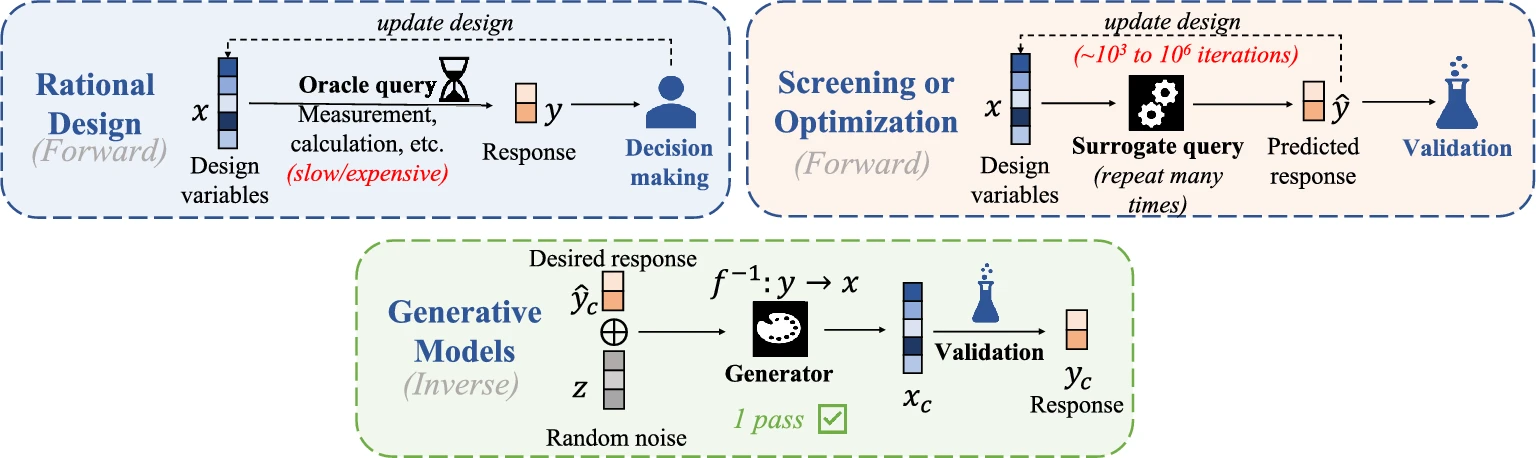
\includegraphics[width=0.96\textwidth]{inversedesign/inverse_fig1.png}
    \caption{A schematic contrasting the design approaches based on (blue) traditional, \emph{rational} forward design, (orange) \emph{screening} forward design, and (blue) \emph{generative} inverse design. Reproduced from \cite{Debnath2023ComparingAlloys} under permission.}
    \label{inverse:fig:designs}
\end{figure}

Most recently, the inverse design paradigm, based around \emph{generative models}, is becoming increasingly popular thanks to further increases in computational power and novel machine learning models, such as generative adversarial networks (GANs) \cite{Goodfellow2020GenerativeNetworks}, which can generate distributions of outputs mimicking prior data, while finding underlying patterns that may be hard to find for even an expert due to high data complexity or quantity. Figure~\ref{inverse:fig:designs} summarizes and contrasts these three design paradigms.


\section{Conditional Generative Design} \label{inverse:sec:cgan}

Materials design tends to focus on the ability to obtain specific key properties, unlike some other ML-related studies like cat or dog image generation, that may be primarily concerned with realistic sampling of the underlying distribution \cite{Ching-YuanBaiJuliaElliott2019GenerativeImages}. Thus, the creation of generator models for materials is usually accomplished with a slightly more elaborate architecture, shown in Figure~\ref{inverse:fig:cgan} and called conditional GAN or \emph{cGAN}, which enables biasing the generated outputs (e.g., compositions) towards specific property values \cite{Mirza2014ConditionalNets, Arjovsky2017WassersteinNetworks}.

\begin{figure}[H]
    \centering
    \includegraphics[width=0.55\textwidth]{inversedesign/inverse_fig2.png}
    \caption{The conditional GAN (cGAN) architecture. It is a variation of the GAN architecture, with the modification that an additional conditioning vector is provided as an input to both $\mathbb{G}$ and $\mathbb{D}$, allowing biasing the model to certain property values. Reproduced from \cite{Debnath2023ComparingAlloys} under permission.}
    \label{inverse:fig:cgan}
\end{figure}



\section{Building and Evaluating Generative Models in ULTERA} \label{inverse:sec:buildinggan}

\subsection{Data and Training} \label{inverse:ssec:datatrain}

Any material design effort requires close integration with existing literature data and scientific techniques to validate generated samples beyond the known set. This is especially true for generative design studies, as the models are specifically tasked with reproducing the underlying distribution. 

Thus, if the underlying data possesses systematically incorrect artifacts, like the ones explored in Chapter \ref{chap:pyqalloy}, one can expect a generative model to learn them. In the case of errors that bring data outside of the typical range, like the ones demonstrated in Figures \ref{pyqalloy:fig:extreme}, \ref{pyqalloy:fig:patternbreak2}, or \ref{pyqalloy:fig:patternbreak2}, the out-of-range values may lead to phenomena like (1) substantial overestimation of errors if they are present in the test set or (2) strongly bias the model to repeatedly generate them for a wide range of latent space samplings because of locally exceptional values. Thus, it becomes critical to use tools like \texttt{PyQAlloy} to ensure that data has few systematic errors present in it.

Furthermore, the data sparsity in terms of compositional (generator output) coverage may strongly contribute to the model overly exploiting some regions under strong conditioning due to insufficient data to establish underlying distribution. Thus, tools like \texttt{nimCSO} become critical in establishing which dimensions of the dataset to model in order to preserve the most knowledge while rejecting data points from which learning may be impossible.

As explored in \citet{Debnath2021GenerativeAlloys}, once a sufficient dataset has been collected from ULTERA, it was passed to the inverse design component of the data ecosystem. To demonstrate novel refractory HEAs with some desired property sets, a cGAN model based on a simple feed-forward NN architecture with four fully connected layers was trained using 529 HEA literature-derived compositions from an early ULTERA Database snapshot. To generate new compositions, the cGAN was conditioned on the shear modulus and fracture toughness values obtained from the empirical model, taking as an input linear combinations of pure element ab initio values from \citet{Chong2021CorrelationAlloys} passed through the \texttt{ULTERA} 's pipeline described in Section \ref{ultera:ssec:autolc}.

The values of these properties were normalized to ensure that the importance of each feature is equivalently reflected in the model. The conditioning values were sampled using the probability distribution of the property values. Batches of normally distributed sixteen-dimensional latent vectors and the sampled conditioning vectors were then provided as input to the generator. One advantage of the adversarial loss of GANs over other competing methods like reconstructive loss of VAEs is the simplicity of the objective function - here, the generator receives the negative critic score as its loss, such that it maximizes the "realism," or the underlying distribution match, of the generated samples. Because the critic is trained in tandem with the generator, there is no need to define a metric for this "realism", which is learned directly from the observed distribution. We used the Wasserstein GAN \cite{Arjovsky2017WassersteinNetworks} loss to avoid vanishing gradients and the unrolled GAN \cite{Metz2016UnrolledNetworks} strategy to avoid mode collapse.

\subsection{Biasing the Predictions to Property Values} \label{inverse:ssec:propbias}

With a trained conditional generative model $\mathbb{G}$, one can begin to assess the effects of the conditioning by, for instance, biasing it to the prediction of certain property values. As demonstrated in \citet{Debnath2021GenerativeAlloys}, this process is not exact; however, it does result in the sampling of regions of the latent space that are better aligned with the desired outcome, thus making it a valuable design tool. As shown in Figure~\ref{inverse:fig:propbias}, one can obtain very different distributions of values in the space of fracture toughness and shear modulus values when different targets are selected. Notably, given targets for which the cGAN had a lot of starting data (point c), it can generally generate narrow distributions, while it struggles in the sparse regions (points a, b, d), highlighting the need for robust training datasets, like one described in Section~\ref{ultera:sec:datadescription}.

\begin{figure}[H]
    \centering
    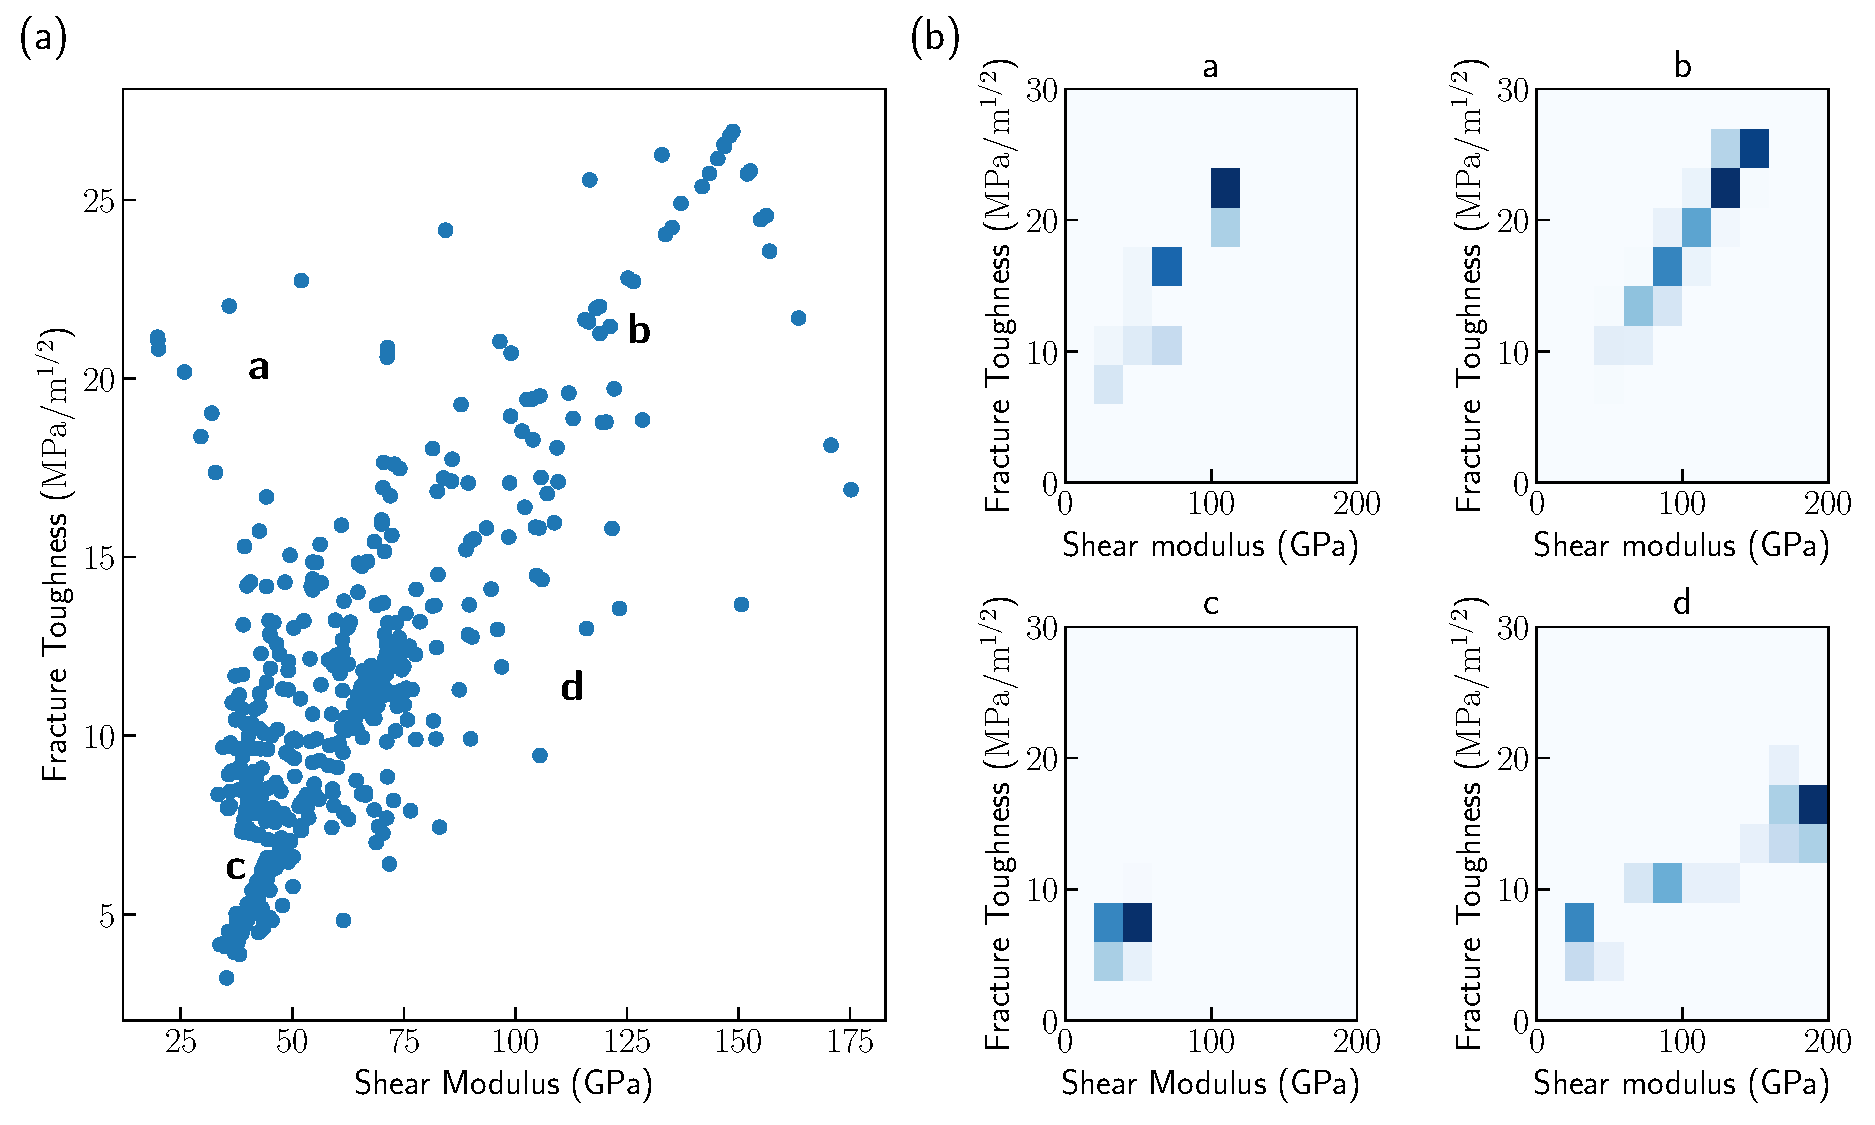
\includegraphics[width=0.85\textwidth]{inversedesign/fixed_cond_multi_points.pdf}
    \caption{(A) Correlation between training shear modulus and fracture toughness values of the compositions from an old version of ULTERA. Points a, b, c, and d represent four conditioning cases of interest. (B) Histograms of shear modulus and fracture toughness for generated compositions. The intensity of blue in the histograms indicates a greater number of compositions with the corresponding values of shear modulus and fracture toughness. In addition to targeted bias, the cross-property correlations are visible. Reproduced from \cite{Debnath2021GenerativeAlloys} under permission.}
    \label{inverse:fig:propbias}
\end{figure}

This effect was observed to usually follow generally expected trends, e.g., in increasing value of shear modulus target causing the frequency of elements like W, Re, and Ru with high elemental shear modulus (173, 150, and 149 GPa, respectively) to increase, while elements like Hf, Mo, and Zr with low elemental shear modulus (30.4, 19.7, and 32.7 GPa) decreased.


\subsection{Biasing the Predictions to Compositional Ranges} \label{inverse:ssec:compbias}

As depicted in Figures \ref{inverse:fig:designs} and \ref{inverse:fig:cgan}, the two spaces sampled by the conditional generative model $\mathbb{G}$ are \emph{latent space} and \emph{property space}. While biasing of the latter, discussed in Subsection \ref{inverse:ssec:propbias}, is the most common approach in material design studies, the biasing of property space has some critical advantages.

For instance, one can utilize it to control the fraction of desired or undesired chemical elements, as shown in \citet{Debnath2023ComparingAlloys} for the case of \ch{W} content control based on recognizing a \emph{concept vector} corresponding to the higher-dimensional direction of high-variance in \ch{W} in the latent space embedding present after training. 

When biasing generative models in such a way, it is critical to consider that, similar to cross-property correlations discussed in Subsection \ref{inverse:ssec:propbias}, biasing the latent space alongside \ch{W} concept vector will also bias all other chemical element contents in the generator outputs.


\section{Demonstrating Generative Design with \texttt{heaGAN}} \label{inverse:sec:heagan}

To create a demonstrator platform for inverse design of high entropy alloys, generative models described in \citet{Debnath2023ComparingAlloys} were extended to several additional properties and deployed as a demonstrator packaged under the name \texttt{heaGAN} and available through interactive cloud notebooks deployed through Binder and GitHub Codespace services, reachable under:

\hspace{36pt}\href{https://cgandemo.ultera.org}{https://cgandemo.ultera.org}

As depicted in Figure \ref{inverse:fig:cgandemo}, the user of the demonstrator is given several parameters to control, including alloy configurational entropy, price, and five physical properties. Each press of the "Generate" button samples a new candidate in a split second.

\begin{figure}[H]
    \centering
    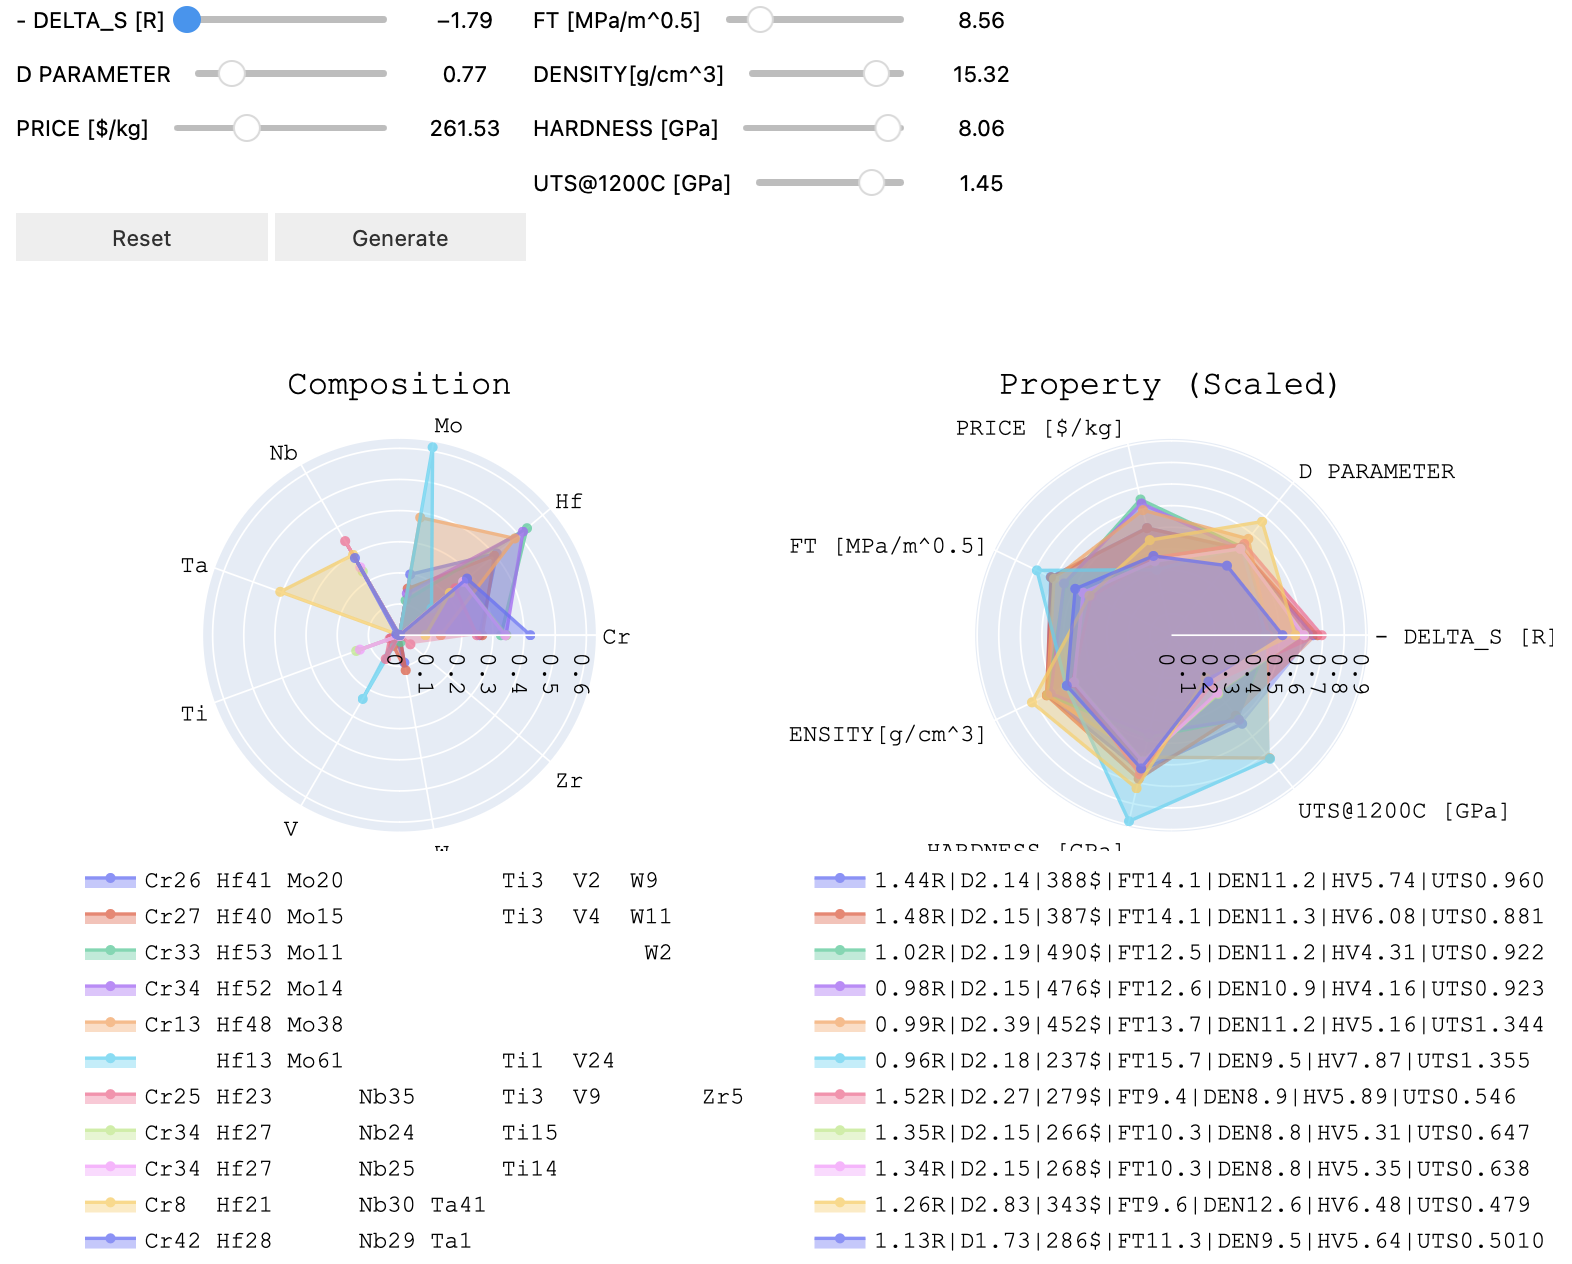
\includegraphics[width=0.7\textwidth]{inversedesign/cgan_demo.png}
    \caption{Printout of the cGAN demonstrator showing several controls user can move to bias the generator to different property values. The depicted plots and lists correspond to a series of biasing values selected semi-randomly to show different values.}
    \label{inverse:fig:cgandemo}
\end{figure}

The forward surrogate models, used to generate inputs for GAN retraining, are stored under \texttt{saved\_surrogates} directory in a free open-source \texttt{ONNX} format to enable both (1) easy swapping for other community models, mostly out-of-the-box and (2) retraining by the end-user on additional datasets. Critically, this can be used to easily implement active learning approaches, dramatically improving the predictive ability of the underlying surrogate models and, by extension, generative models trained on them. As shown in Figure \ref{inverse:fig:activelearn} depicting hardness surrogate refitting, just three data points can be used to fit such a model to a new ternary chemical system.

\begin{figure}[H]
    \centering
    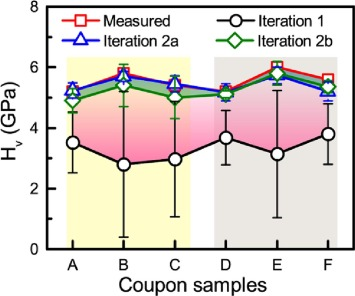
\includegraphics[width=0.4\textwidth]{inversedesign/inverse_active.jpg}
    \caption{Vickers hardness predicted for 6 \ch{Mo-Nb-W} alloys in \cite{Li2024DesignExperiments} generated by a cGAN model both before the first measurement and after just 3 measurements (first or second iteration) become available. The original dataset contained no ternary of interest nor its binaries nor many related systems. Reproduced from \cite{Li2024DesignExperiments}.}
    \label{inverse:fig:activelearn}
\end{figure}



%\section{Discussion} \label{inverse:sec:discussion}




\printbibliography[heading=subbibintoc]